\documentclass[a4paper,11pt,UTF8]{bitbook}
\usepackage{ctex}
\usepackage{amsmath,amsthm,amssymb,amsfonts}
\usepackage{amsmath}
\usepackage[a4paper]{geometry}
\usepackage{graphicx}
\usepackage{microtype}
\usepackage{siunitx}
\usepackage{booktabs}
\usepackage[colorlinks=false, pdfborder={0 0 0}]{hyperref}
\usepackage{cleveref}
\usepackage{esint} 
\usepackage{graphicx}
\usepackage{ragged2e}
\usepackage{pifont}
\usepackage{extarrows}
\usepackage{mathptmx}
\usepackage{float}
\usepackage{caption}
\usepackage{bm}
\usepackage{multirow}
\usepackage{subfigure}
\usepackage{titlesec}
\captionsetup[figure]{name={Figure}}
%opening
\title{科学计算引论作业(七)}
\author{谢悦晋 \quad U202210333}
\date{Nov 13rd, 2023 }
\begin{document}
\maketitle
\textbf{5.1} 试分别利用中矩公式、梯形公式及 Simpson 公式计算定积分
$$
I=\int_0^{\frac12}\exp(3x)\cos2x\mathrm{d}x,
$$
并比较其计算精度。

\noindent 解:

中矩形公式:
$$
	\int_{0}^{\frac{1}{2}}\exp(3x)\cos 2x\mathrm{d}x\approx(\frac12-0)f(\frac14)=0.9289211490504564
$$

梯形公式:
$$
\int_{0}^{\frac{1}{2}}\exp(3x)\cos 2x\mathrm{d}x\approx(\frac12-0)\frac{f(\frac12)+f(0)}{2}=0.8553667347219239
$$

Simpson公式:
$$
\int_{0}^{\frac{1}{2}}\exp(3x)\cos 2x\mathrm{d}x\approx\frac{\frac12-0}{6}(f(0)+4f(\frac14)+f(\frac12))=0.9044030109409457
$$

比较准确的解为$I=0.9082171883002617$, $\varepsilon=1.0083236338112719e-14$,可以看出Simpson公式精度最好

\textbf{5.2} 试确定下面求积公式
$$
\int_{-1}^1f(x)\mathrm{d}x\approx a[f(x_0)+f(x_1)+f(x_2)],
$$
使其具有 3 次代数精度,并由该公式计算定积分:
$$
	\int_{-1}^1\frac{x\sin x}{\sqrt{1+x^2}}\mathrm{d}x
$$
\noindent 解:

由代数精度的定义可以得到以下方程:
$$
\begin{cases}
	 a(1+1+1)=2\\
	 a(x_0+x_1+x_2)=0\\
	 a(x_0^2+x_1^2+x_2^2)=\dfrac{2}{3}\\
	 a(x_0^3+x_1^3+x_2^3)=0\\
	 a(x_0^4+x_1^4+x_2^4)\neq0
\end{cases}\Rightarrow
\begin{cases}
	a=\dfrac{2}{3}\\
	x_0=-\dfrac{\sqrt{2}}{2}\\
	x_1=0\\
	x_2=\dfrac{\sqrt{2}}{2}\\
\end{cases}
$$

计算结果如下:

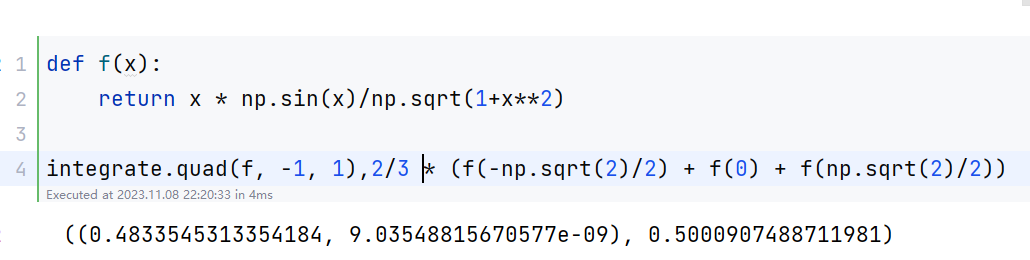
\includegraphics[width=1\textwidth]{5.2_1}

\textbf{5.5} 试构造两点 Gauss 型求积公式
$$
	\int_{-1}^1f(x)\mathrm{d}x\approx A_0f(x_0)+A_1f(x_1),
$$

并由此计算积分:
$$
	\int_0^1\sqrt{1+2x}\mathrm{d}x
$$
\noindent 解:

由代数精度的定义可以得到以下方程:
$$
\begin{cases}
	A_0+A_1=2\\
	A_0x_0+A_1x_1=0\\
	A_0x_0^2+A_1x_1^2=\dfrac{2}{3}\\
	A_0x_0^3+A_1x_1^3=0\\
\end{cases}\Rightarrow
\begin{cases}
	A_0=1\\
	A_1=1\\
	x_0=-\dfrac{1}{\sqrt{3}}\\
	x_1=\dfrac{1}{\sqrt{3}}\\
\end{cases}
$$

对于原积分不能直接使用上述的得到的Gauss积分公式,我们进行一个积分变换:
$$
	\int_0^1\sqrt{1+2x}\mathrm{d}x\xlongequal{t=2x-1}=\frac12\int_{-1}^1\sqrt{2+t}\mathrm{d}t
$$

计算结果如下:

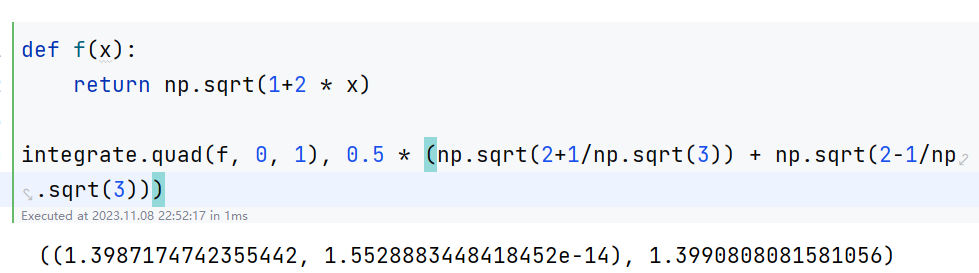
\includegraphics[width=1\textwidth]{5.5_1}

\textbf{5.7} (实验题) 分别用变步长梯形求积公式和 Romberg 算法计算椭圆积分
$$
	\int_0^\pi\frac{\sqrt{2}}{(1+\sin^2x)\sqrt{2-\sin^2x}}\mathrm{d}x
$$

要求其逼近值 $T_k,T_k^{(0)}$ 的计算精度分别满足 $|T_k-T_{k-1}|<10^{-12}$ 和$|T_k^{(0)}-T_{k-1}^{(0)}|<10^{-12}$.

\noindent 解:

结果如下:
\begin{figure}[H]
	\centering
	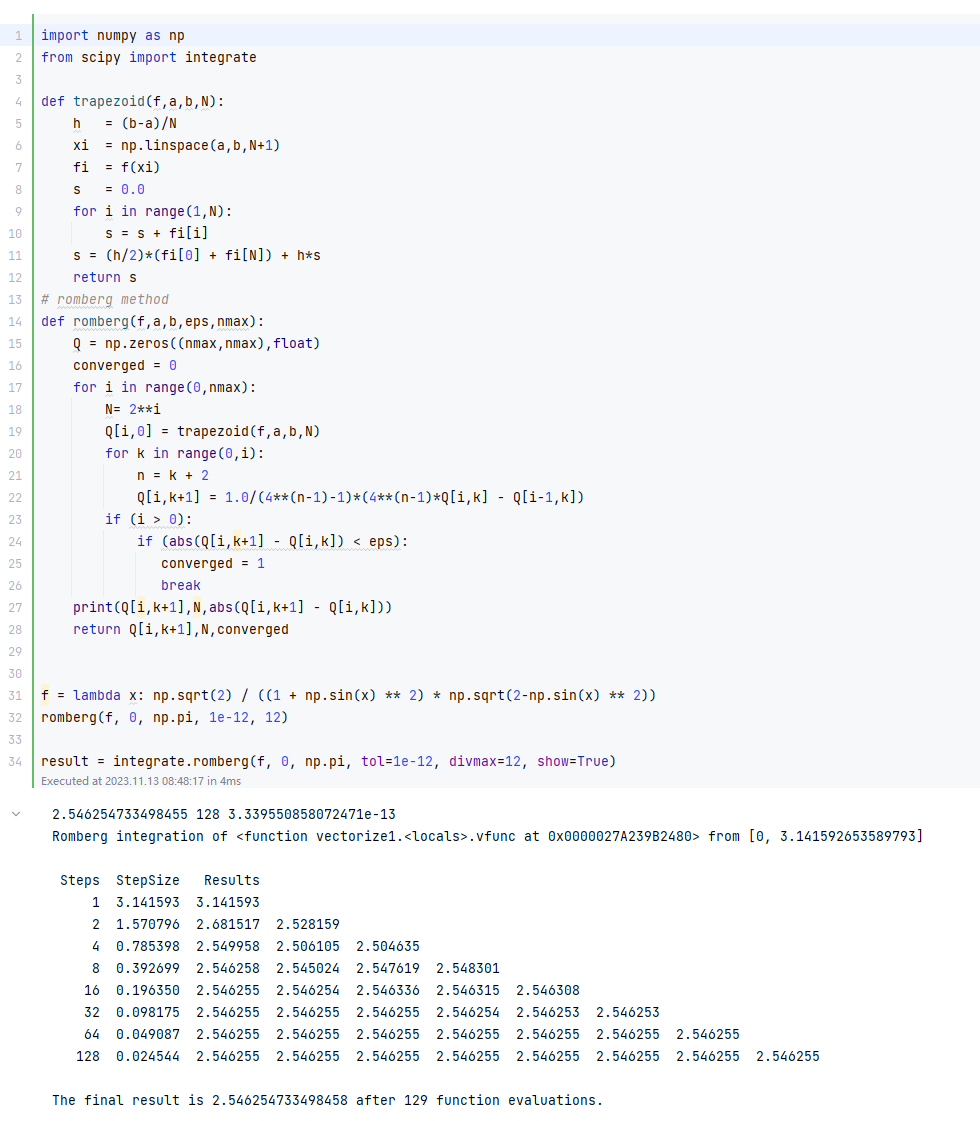
\includegraphics[width=0.7\textwidth]{5.7}
\end{figure}

\end{document}    